\chapter{Imagerie de flux 4D du système cardiovasculaire de la souris rehaussée par des nanoparticules de fer avec une séquence UTE.}
\setlength{\footskip}{50pt}
\chaptermark{Imagerie 4D de mesure de flux}
\label{Chap6}
\section{Contexte}

Les méthodes développées précédemment au cours de cette thèse permettent d'obtenir des informations anatomiques et fonctionnelles précises. D'autres paramètres peuvent être intéressant à explorer dans le cas de pathologie cardiovasculaire comme la mesure de flux. L'imagerie 4D (3D + t) de flux est une stratégie particulièrement intéressante car elle permet à partir d'une même acquisition d'obtenir tout au long du cycle cardiaque : des images en magnitude pour visualiser des modifications anatomiques  \cite{Eriksson:2013aa}, des images de contraste de phase pour visualiser les flux anormaux \cite{Velikina:2010hc}, des cartes de vitesse des flux \cite{Garcia:2014aa} qui peuvent ensuite être utilisée pour calculer d'autres paramètres hémodynamiques comme la différence de pression \cite{Tyszka:2000aa,bock2011vivo} ou les contraintes de cisaillement sur les parois des vaisseaux (Wall Shear Stress : WSS)\cite{Zhao:2009ng} etc. Cette méthode apparait donc comme un important outil diagnostique en médecine mais son utilisation en routine clinique reste encore aujourd'hui fortement limité en particulier à cause des temps d'acquisitions requis important (10 à 20 minutes sur un coeur entier).

Les problématiques liées à l'utilisation de cette méthode sont exacerbées dans le cas de l'imagerie préclinique et en particulier chez la souris. En effet, le faible signal ainsi que le faible nombre de canaux des antennes limites l'utilisation des méthodes d'accélération parallèle ce qui augmente fortement les temps d'acquisitions des séquences de quantification de flux 4D par imagerie de phase. De plus, la présence de flux important (> 1 m/s) dans des vaisseaux de petites tailles et avec une anatomie complexe a pour effet de favoriser le déphasage intravoxel des spins et donc l'apparition d'artéfacts de perte de signal sur les images. Pour réduire ces artéfacts la méthode la plus simple est de réduire le temps d'écho \cite{staahlberg1994pulse,OBrien:2008aa}. L'amélioration des systèmes de gradients que ce soit en terme d'intensité ou de temps de montée ont permis d'atteindre des valeurs de temps d'écho de 2 à 4 ms en imagerie cartésienne conventionnelle.

L'utilisation de trajectoire non-cartésienne permet d'atteindre des temps d'écho encore plus faible ainsi que de réduire la sensibilité aux artéfacts de flux. O'Brien et al  \cite{OBrien:2009ul} ont montré que l'utilisation une séquence 2D de mesure de flux basé sur une trajectoire radiale UTE permettait en atteignant un TE de 0.6 ms d'obtenir des mesures plus précises grâce à la réduction des artéfacts de déphasage des spins dans le cas des flux ayant une vitesse rapide.  Janiczek et al \cite{Janiczek:2011qm} ont développé et appliqué une séquence 3D de mesure de flux de type Stack-Of-Star spiral sur la crosse aortique d'une souris qui, grâce à l'effet temps-de-vol, permet d'obtenir un rapport signal-sur-bruit suffisant pour dériver le WSS. Ils ont montré dans cette étude que cette trajectoire permet d'obtenir un meilleur signal-sur-bruit que la séquence cartésienne et est moins sensible aux artéfacts de flux dans les régions avec une vitesse rapide et incurvés. Récemment Kadbi et al \cite{Kadbi:2014uq} ont étudié l'utilisation d'une séquence 3D Stack-Of-Star UTE pour la quantification des flux sténotiques et ont montré que cette stratégie permet d'obtenir des résultats en accord avec les mesures cartésiennes pour les flux lents mais surtout de meilleurs résultats dans les cas des flux rapides.

Une des possibilités pour atteindre des temps d'écho encore plus court est d'utiliser une trajectoire 3D UTE combinée à une impulsion radiofréquence non-sélective. Bien qu'il soit nécessaire d'ajouter des gradients bipolaires dans le cas d'une séquence de mesure de flux, la séquence 4D UTE de mesure de flux permet d'atteindre des temps d'échos inférieurs à 0,5 ms. De plus l'absence de gradient d'encodage selon la direction de coupe permet de réduire la sensibilité aux artéfacts de flux de cette séquence par rapport aux approches Stack-Of-Star. 

Cependant, dans le cas de l'imagerie cardiaque il n'est pas possible d'obtenir d'effet temps-de-vol comme expliqué dans les parties précédentes de cette thèse. Or le bruit des cartes de vitesse des flux est inversement proportionnel au signal sur les images en magnitude. L'approche employée est donc une fois de plus d'utiliser l'injection d'un agent de contraste à base de nanoparticule de fer qui permettra d'obtenir un fort signal du sang grâce au faible temps d'écho obtenu avec la séquence employée.

Au cours de ce chapitre, la méthode d'encodage de flux sera rapidement présentée ainsi que son implémentation à l'aide d'une séquence 3D ciné UTE. Les mesures de vitesse effectuée avec cette méthode seront comparées par rapport à une séquence cartésienne sur un fantôme de flux. L'impact de la réduction des valeurs $T_2*$ dans le cas de l'utilisation de nanoparticules de fer sur la mesure des vitesses sera évalué. Ce travail est en cours de développement et nous présenterons dans la dernière partie de ce chapitre, les résultats préliminaires obtenus sur un modèle de souris d'hypertension artérielle pulmonaire.

\section{Stratégie de mesure de flux 4D}

\subsection{Introduction à la mesure de flux par imagerie de phase}

\subsubsection{Encodage des vitesses}

La quantification des flux grâce à la phase en IRM utilise l'ajout d'un gradient bipolaire entre l'excitation radiofréquence et la lecture du signal pour encoder la vitesse des flux. La figure \ref{fig:PhaseSpins} montre l'effet du gradient bipolaire d'encodage de vitesse sur des spins fixes et mobiles et en particulier l'accumulation de phase. On observe qu'à la fin du gradient bipolaire la phase des spins fixes retourne à sa position initiale alors les spins mobiles accumulent une phase qui est directement proportionnelle à leurs vitesses.

\begin{figure}[H]
\centering
\line(1,0){400} \\
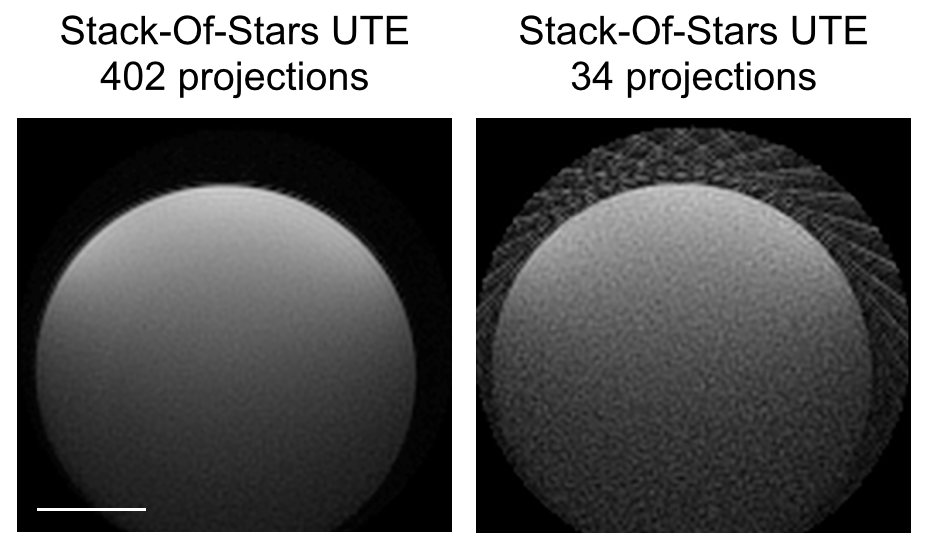
\includegraphics[scale=0.5]{./figure/chap6/Fig1.png}
\caption[Effet du gradient bipolaire]{\label{fig:PhaseSpins} Représentation schématique de l'accumulation de la phase au cours du temps dans le cas de spins fixes et de spins mouvants sous l'influence d'un gradient bipolaire. L'accumulation de phase subit par les spins mouvants est proportionnelle à leurs vitesse. }
\line(1,0){400} \\ 
\end{figure}
Si l'on défini la position des spins en fonction du temps de la manière suivante :
\begin{align}
x(t)=x(0) + x_1 t +\frac{1}{2!} x_2 t^2 + ... + \frac{1}{n!} x_n t^n
\end{align}
où $x_1$ représente la vitesse du spin et $x_2$ son accélération selon la direction du gradient bipolaire. Alors la phase accumulée peut se calculer grâce à l'équation suivante :

\begin{align}
\phi (T) &= \gamma \int_0^T G(t) x(t) dt \\
			 &= \gamma (m_0 x(0) + m_1(T) x_1 + ...)
\end{align}
où m représente le moment du gradient. 
	Dans notre cas, on désire mesurer la vitesse des flux, il est donc nécessaire que le moment de gradient $m_0$ soit égale à 0. Cela se traduit géométriquement à ce que l'aire globale du gradient bipolaire soit égale à 0 (ce qui est le cas dans la figure \ref{fig:PhaseSpins}). Le premier moment $m_1$ représenté dans cette figure peut être calculé directement :
	
	\begin{equation}
	\begin{split}
	m_1 &= \int_{t=0}^{T_L} -G \ t \ dt  + \int_{t=T}^{T+T_L} -G \ t \ dt  \\
			&= \frac{G}{2}\left(-T_L^2+(T+T_L)^2-T^2\right) \\
			&=G \ T_L \ T \\
			& = A \ T
	\end{split} 
	\end{equation}	
où $T_L$ correspond à la durée d'un lobe, T à la durée entre le départ des deux lobes et A à l'aire d'un lobe. Ce résultat est ici démontré à partir d'un gradient rectangulaire, mais il est généralisable à n'importe quelle forme de gradient bipolaire en les décomposant en une infinité de rectangle avec une largeur infinitésimale. Ce résultat s'applique donc aussi aux gradients avec une forme trapézoïdale qui est la forme de gradient la plus couramment utilisée dans les séquences.

L'accumulation de phase pour un groupe de spin ayant une vitesse constante est donc égale à :
\begin{equation}
\Phi = \gamma A \ T \ v
\end{equation}
et en modifiant la valeur de l'intensité du gradient bipolaire ou sa durée d'application il est donc possible de modifier l'accumulation de phase des spins mouvants en fonction de leurs vitesses.

\subsubsection{Quantification de la vitesse par imagerie de phase}

Pour mesurer la vitesse des spins, il est nécessaire de supprimer la phase statique des tissus produite par les hétérogénéités du champ magnétique $B_0$. La méthode généralement employée consiste à acquérir deux images avec des intensités de gradient bipolaire différentes et de soustraire ensuite leurs phases. Les deux méthodes les plus employés sont représentées dans la figure \ref{fig:MethodeGradientBip}. La méthode (a) permet de diviser d'un facteur 2 l'intensité maximum des gradients d'encodage des vitesses par rapport à la méthode (b). La méthode (b) est encore souvent utilisée car elle permet d'utiliser l'image sans gradient bipolaire comme image de référence en magnitude et qui est donc moins sensible aux artéfacts de déphase de flux.
\begin{figure}[h]
\centering
\line(1,0){400} \\
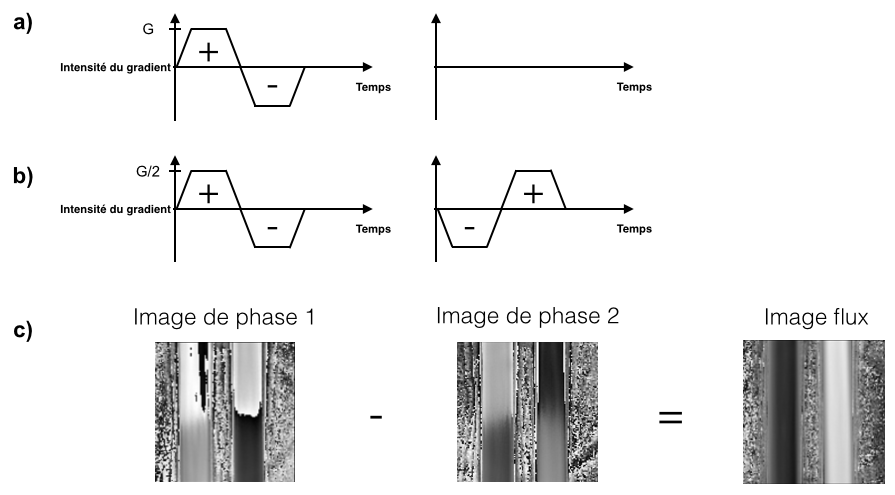
\includegraphics[scale=0.5]{./figure/chap6/Fig2.png}
\caption[Méthodes gradient bipolaire]{\label{fig:MethodeGradientBip} Représentation de l'intensité des gradients bipolaires utilisés pour deux images dont la soustraction permet d'obtenir une image de mesure de flux où seul la phase crée par les vitesses des spins est présente. Les deux méthodes représentées permettent d'obtenir la même amplitude de codage des vitesses définies par $\Delta m_1 = m_1(image1) - m_1(image2)$. La méthode \textbf{(a)} consiste à inverser la polarisation des gradients bipolaires entre les deux images dont l'intensité est égale à G/2. La méthode \textbf{(b)} consiste à recueillir une image avec une intensité G et la seconde sans gradient bipolaire (mais en maintenant le TE de la séquence). }
\line(1,0){400} \\ 
\end{figure}

Lorsque la vitesse des spins est trop importante, il est possible que leurs phases $| \Phi | > \pi$, on observe alors un repliement de la phase qui est problématique pour déterminer la vitesse des spins. Le paramètre de vitesse d'encodage des spins souvent noté VENC pour "Velocity ENCoding" a donc été inventé et est généralement exprimé en cm/s. Celui-ci est fixé par l'utilisateur et correspond à la vitesse maximum qui peut être encodée sans observer de repliement de la phase. Il est donc défini à partir du moment $\Delta m_1=m_1(image_1)-m_1(image_2)$ :
\begin{align}
\text{VENC} = \frac{\pi}{\gamma | \Delta m_1 |}
\end{align} 

En réalité, l'utilisateur va définir le paramètre VENC et l'intensité/durée des gradients bipolaires est alors calculée en conséquence pour permettre d'obtenir l'encodage des vitesses correspondantes des spins. Dans le cas des gradients trapézoïdaux présentées dans la figure \ref{fig:MethodeGradientBip} qui sont ceux implémentées dans cette séquence, l' intensité des gradients d'encodage G est définie par :

\begin{align}
G = \frac{\pi}{2 \gamma \ A_n \ T \ \text{VENC}}
\end{align}
où $A_n$ correspond à l'aire normalisée pour que le maximum soit égale à 1. En posant r le temps de montée et de descente des gradients et d la durée du plateau de la figure \ref{fig:MethodeGradientBip}, on obtient a alors $A_n = d+r$ et $T = d+2r$.

La valeur de VENC choisi par l'utilisateur doit être supérieure à la vitesse maximum pour éviter le repliement mais doit aussi soit aussi être relativement assez proche des vitesses à observer car le paramètre de vitesse-sur-bruit dans les cartes de vitesse (l'équivalent du signal-sur-bruit) suit une loi du type :
\begin{align}
\text{VNR} \propto \frac{V}{\text{VENC}}\text{SNR}
\end{align}
On observe que le VNR est inversement proportionnel  à la valeur de VENC donc plus le choix du VENC est faible (et donc proche des valeurs que l'on souhaite observer) meilleur seront les mesures. Généralement le paramètre VENC est choisi de manière à être 30$\%$ inférieur à la vitesse maximum espérée. De plus on observe aussi que ce paramètre VNR est proportionnel au SNR, il est donc important d'obtenir des images avec un bon rapport SNR dans les régions anatomiques que l'on souhaite quantifier.

\subsubsection{Antennes multicanaux et reconstruction des images de mesure des flux}

La méthode de référence pour reconstruire des données obtenues avec une antenne multicanaux et l'utilisation d'une la somme des carrés. Le problème de cette stratégie est la perte des informations de phase dans l'image finale.

Si on défini 2 images complexes $I_1$ et $I_2$ qui sont acquises avec l'une des stratégies de contraste de phase définie dans la partie précédente. Ces images peuvent être représentée en utilisant leurs magnitude (A) et phase ($\Phi$) respective :
\begin{equation}
\begin{split}
I_1= A_1 . e^{i \Phi_1} \\
I_2= A_2 . e^{i \Phi_2}
\end{split}
\end{equation}
La carte de contraste de phase $\Delta \Phi$ pour une antenne à un élément peut alors se calculer de la manière suivante :
\begin{equation}
\begin{split}
\Delta \Phi &= arg(I_1 \cdot I_2^*) \\
				  &= arg(A_1 \cdot A_2 \cdot e^{i(\Phi_1 - \Phi_2)}) \\
				  &= \Phi_1-\Phi_2
\end{split}
\end{equation}
Cette équation peut être étendue à des données recueillies avec une antenne multicanaux où l'opération de différence de phase est effectuée après la combinaison de tout les canaux individuellement.

\begin{equation}
\begin{split}
\Phi_1 &= arg( \sum_1^n  A_{1n} \cdot e^{i \Phi_{1n}}) \\
\Phi_2 &= arg( \sum_1^n  A_{2n} \cdot e^{i \Phi_{2n}}) \\
\Delta \Phi &= \Phi_1 - \Phi_2
\end{split}
\end{equation}

Une autre méthode disponible décrite par Bernstein et al \cite{bernstein1994reconstructions} consiste à effectuer l'opération de différence de phase individuellement pour chaque canal puis de combiner les données pour générer la carte de phase :

\begin{align}
\Delta \Phi = arg(\sum_1^n A_1 \cdot A_2 \cdot e^{i(\Phi_1n - \Phi_2n)})
\end{align}

Dans ce chapitre, la méthode employée est la méthode de Bernstein qui s'avère donner de meilleur résultat.

\subsection{Chronogramme de la séquence 3D UTE de contraste de phase}

\begin{figure}[H]
\centering
\line(1,0){400} \\
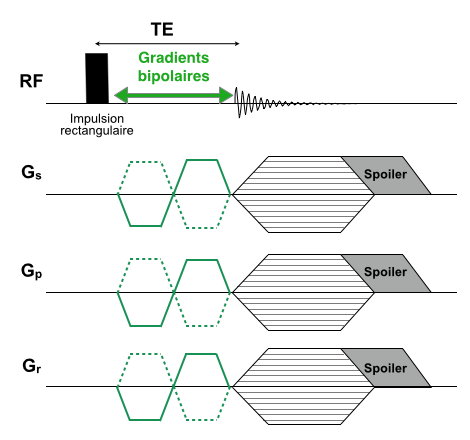
\includegraphics[scale=0.5]{./figure/chap6/Fig3.png}
\caption[Chronogramme 4D flux]{\label{fig:Chrono4DFlux} Chronogramme de la séquence 4D UTE de contraste de phase. Des gradients bipolaires (en vert) sont présents entre l'excitation radiofréquence non-sélective et la lecture du signal. La polarité et l'intensité des gradients bipolaires est définies en fonction de la méthode d'encodage des vitesses employée.}
\line(1,0){400} \\ 
\end{figure}

La séquence développée au cours de ce travail, illustrée par la figure \ref{fig:Chrono4DFlux}, est basée sur la séquence 3D UTE présentée dans le chapitre \ref{Chap4} à laquelle on a ajouté des gradients bipolaires entre l'impulsion de radiofréquence et la lecture du signal (indiqué en vert).
Les gradients bipolaires utilisés dans ce travail sont des gradients trapezoidaux définis par leurs temps de monté r, la durée du plateau d et l'intensité maximum G. La polarité du premier lobe peut être positive ou négative correspondant respectivement aux traits pointillés et pleins sur la figure.

Pour mesurer la vitesse selon les 3 directions de l'espace, il est nécessaire d'encoder les vitesses selon les 3 axes ce qui requiert au minimum 4 acquisitions avec des combinaisons de gradient bipolaire différentes. Plusieurs combinaisons de gradient bipolaire sont à disposition et ont été implantées dans la séquence. Ces différentes combinaisons de polarité des gradients des 3 axes sont présentées dans la figure \ref{fig:EncFlux} : 4-points standard, 4-points symétrique, 4-points Hadamard. 

\begin{figure}[H]
\centering
\line(1,0){400} \\
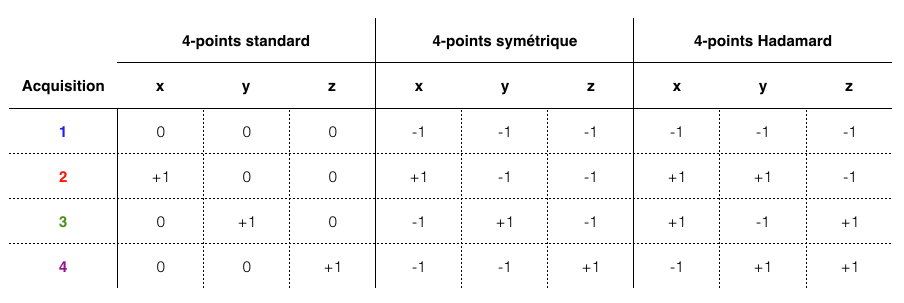
\includegraphics[scale=0.5]{./figure/chap6/Fig4.png}
\caption[Méthode encodage flux]{\label{fig:EncFlux} Tableau représentant la polarité des gradients bipolaires pour 3 méthodes : 4-points standard, 4-points symétrique et 4-points Hadamard. Pour obtenir le même encodage des vitesses pour la méthode standard, l'intensité des gradients bipolaires est 2 fois plus importante que pour les deux autres méthodes.}
\line(1,0){400} \\ 
\end{figure}

Pour obtenir les cartes de vitesses après la reconstruction de chaque acquisition individuellement, la combinaison des données est différentes en fonction des méthodes. Pour la méthode standard et symétrique, les cartes de vitesses ($V_x,V_y,V_z$) sont obtenues en combinant les cartes de phase des acquisitions, noté $Acq_x$ selon la méthode suivante :

\begin{equation}
\begin{split}
V_x = (Acq_2-Acq_1) \frac{\text{VENC}}{\pi} \\
V_y = (Acq_3-Acq_1 ) \frac{\text{VENC}}{\pi}\\
V_z = (Acq_4-Acq_1 ) \frac{\text{VENC}}{\pi}
\end{split}
\end{equation}

Pour la méthode d'encodage Hadamard, la combinaison des acquisitions utilisent toutes les données :

\begin{equation}
\begin{split}
V_x = (-Acq_1+Acq_2+Acq_3-Acq_4) \frac{\text{VENC}}{\pi} \\
V_y = (-Acq_1+Acq_2-Acq_3+Acq_4 ) \frac{\text{VENC}}{\pi}\\
V_z = (-Acq_1-Acq_2+Acq_3+Acq_4 ) \frac{\text{VENC}}{\pi}
\end{split}
\end{equation}

Durant ce travail, les méthodes 4-points symétrique et Hadamard ont été favorisées car elles permettent de réduire l'intensité maximum des gradients d'un facteur 2 et donc, pour obtenir la valeur VENC désirée, de diminuer la durée des gradients permettant de réduire le TE de la séquence. Le choix définitif s'est porté sur la méthode symétrique car la plage dynamique des vitesses qui peut être mesurée avec la méthode Hadamard sans obtenir de repliement n'est pas indépendante de la direction de la vitesse des flux. Il est donc possible d'obtenir un repliement de la phase si la vitesse est supérieur à $v=\text{VENC}/\sqrt{2} $ selon 2 directions d'encodage des vitesses \cite{Pelc:1991aa} contrairement à la méthode d'encodage symétrique.

\subsection{Stratégie d'encodage 4D de vitesse des flux}


La séquence est synchronisée prospectivement pour mesurer la vitesse des flux. Au cours d'un cycle cardiaque NCine phases sont reconstruites, chaque phase est composée de 4 signaux IRM permettant d'encoder la vitesse selon les 3 dimensions. Tout les signaux recueillis au cours du même battement de coeur ont la même trajectoire, celle-ci est défini selon la méthode présentée dans le chapitre \ref{Chap4}. La couleur des signaux IRM qui sont représentée sur la figure \ref{} permet de représenter la polarité des gradients bipolaires qui sont utilisés en accord avec les couleurs des acquisitions représentées dans la figure \ref{fig:EncFlux}. L'ordre d'encodage des signaux IRM dans chaque phase cardiaque est déplacé d'une étape à chaque battement de coeur. 

Cette stratégie permet de recueillir à chaque battement de coeur les projections permettant d'encoder les trois directions avec une même trajectoire. Le changement d'ordre d'encodage permet de moyenner le mouvement et les modifications de vitesse sur la durée de la phase cardiaque qui sera reconstruite.

\begin{figure}[H]
\centering
\line(1,0){400} \\
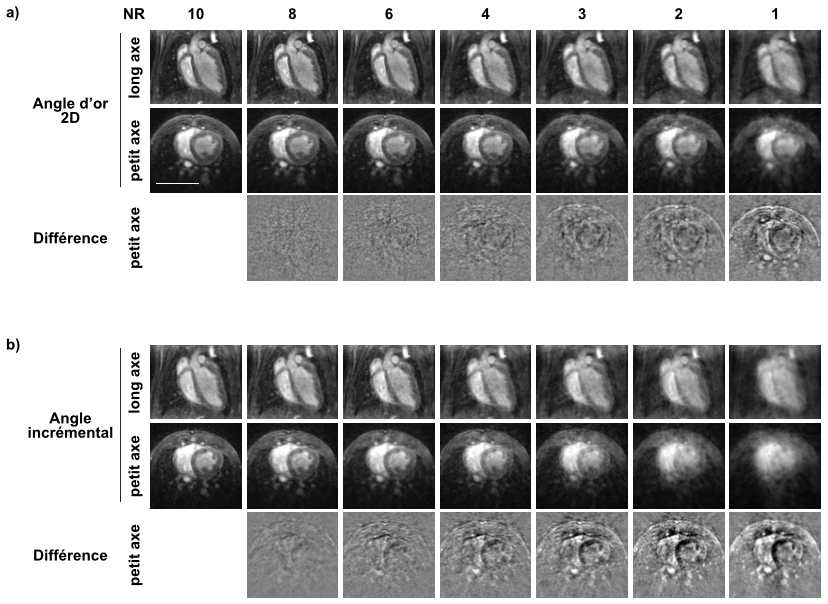
\includegraphics[scale=0.5]{./figure/chap6/Fig5.png}
\caption[Schéma acquisition flux]{\label{fig:SchemaAcqFlux} Schéma d'acquisition synchronisée prospectivement sur le rythme cardiaque de la séquence 4D UTE de mesure de flux.}
\line(1,0){400} \\ 
\end{figure}

\subsection{Correction des erreurs de phase/vitesse}

Les erreurs observées en imagerie de flux proviennent principalement de 3 sources : les courants de Foucault \cite{Walker:1993aa}, les gradients concomitants \cite{Bernstein:1998aa} et les distorsions du champ de gradient provenant de la géométrie des bobines de gradient. \cite{Markl:2003aa}. Diverses méthodes existent pour corriger ces erreurs. Dans ce chapitre la méthode décrite par Chernobelsky et al \cite{Chernobelsky:2007aa} a été implémentée car elle permet de corriger les erreurs provoquées par les courants de Foucault et les gradients concomitants. Cette méthode consiste à appliquer la même séquence d'imagerie (avec les même paramètres) sur un fantôme homogène statique, puis de soustraire les cartes de vitesse obtenues avec ces données aux cartes obtenues \textit{in vivo}. 

Un exemple d'application de cette stratégie de correction est présenté dans la figure \ref{fig:CorrectionPhase} où l'on observe, sur un fantôme de flux, la présence d'une erreur linéaire sur la carte de vitesse non-corrigée. Après soustraction avec l'image acquise sur le fantôme statique, l'erreur linéaire est corrigée.% et l'on observe seulement les variations de vitesse provenant de la difficulté à placer le trait de mesure au centre du tube.

Lorenz et al \cite{Lorenz:2014aa} ont montrés que cette stratégie permettait de grandement améliorer les résultats dans le cadre de l'utilisation de représentation des trajectoires des flux. Ils ont aussi quantifiée que l'impact des erreurs provenant des distorsions de champ de gradient était faible sur un imageur clinique. Or en imagerie préclinique le diamètre de l'aimant est plus faible ce qui réduit d'autant plus ce type d'erreur par rapport à l'étude menée par Lorenz.

\begin{figure}[H]
\centering
\line(1,0){400} \\
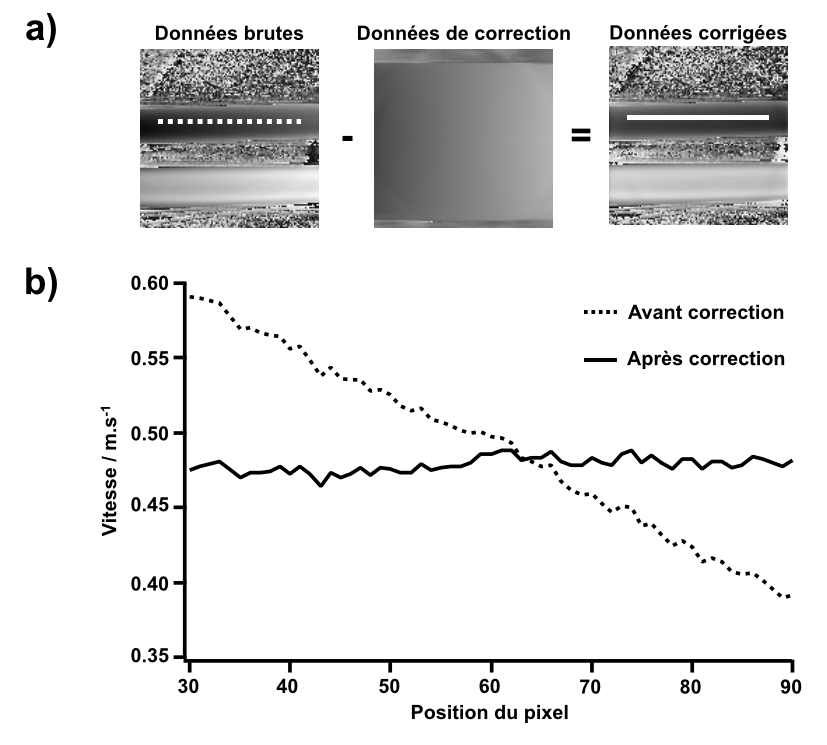
\includegraphics[scale=0.5]{./figure/chap6/Fig6.png}
\caption[Correction de la phase]{\label{fig:CorrectionPhase} Correction des erreurs de phase par soustraction des cartes de vitesse avec une carte de vitesse recueillie sur un fantôme homogène. Le signal mesuré au niveau des lignes pointillées et pleines est représenté sur le graphique.}
\line(1,0){400} \\ 
\end{figure}

\section{Validation \textit{in vitro}}

La séquence a été validée sur un fantôme de flux constitué d'un tube d'eau statique et d'un tube droit effectuant un aller-retour dans le champ de vue dans lequel circule de l'eau avec du chlorure de manganèse ($\text{MnCl}_2$) à différentes concentrations permettant d'imiter l'effet $r_2*$ des nanoparticules de fer. Le chlorure de manganèse est ici utilisé pour une question de coût.
%correspondant respectivement à un $T_2 \approx 393/6/3/1,5/1/0,8 ms$

La première étape a été de vérifier la robustesse des mesures de vitesse à la diminution des valeurs de $T_2*$ qui apparait après l'injection d'un agent de contraste à base de nanoparticule de fer. Pour cela, la vitesse dans le tube a été mesurée pour des concentrations en $\text{MnCl}_2$ de 0, 1, 2, 4, 6, 8 mM et des valeurs de VENC de 1.2, 1.0, 0.8, 0.6 m/s. Le débit du flux a été fixé durant toutes les acquisitions pour générer une vitesse moyenne de 0.258 m/s. Les vitesses ont été quantifiée avec la séquence 3D UTE ainsi qu'avec une séquence FLASH de mesure de flux avec les même paramètres d'acquisition mis à part un TE de 2,3 ms contrairement à l'acquistion UTE qui a un TE de 0,571 ms. Les résultats sont présentées sur la figure \ref{fig:FluxFantT2}. Les mesures effectuées avec la séquence UTE ($v=0.267 \pm 0.0063 m/s$) montrent une très faible dispersion que ce soit en fonction de la valeur VENC ou de la concentration en manganèse contrairement aux mesures effectuées avec le séquence FLASH ($v=0.284 \pm 0.065 m/s$). La dispersion avec la séquence FLASH n'est pas extrêmement sensible à l'augmentation de concentration en manganèse sur nos mesures et une partie peut s'expliquer par l'aspect pulsatile de la pompe. La séquence UTE étant très peu sensible à ce type d'artéfact les mesures montrent donc une forte reproductibilité.

\begin{figure}[H]
\centering
\line(1,0){400} \\
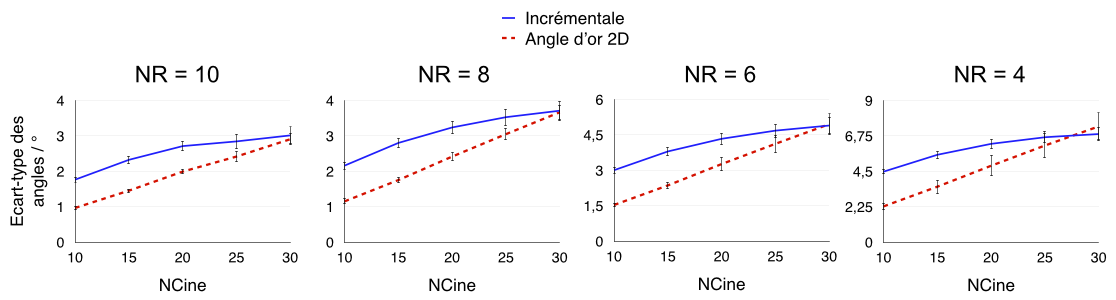
\includegraphics[scale=0.5]{./figure/chap6/Fig7.png}
\caption[Mesure du flux en fonction du T2*]{\label{fig:FluxFantT2} Mesure des vitesses sur un fantôme de flux effectuée avec une séquence FLASH et UTE en fonction de la concentration en $\text{MnCl}_2$ (0, 1, 2, 4, 6, 8 mM) et pour différentes valeurs de VENC (1.2, 1.0, 0.8, 0.6 m/s).}
\line(1,0){400} \\ 
\end{figure}

La deuxième partie de l'étude sur fantôme a pour objectif de vérifier la linéarité des mesures de vitesse. Les mesures ont été effectuées avec les même paramètres pour la séquence FLASH et UTE avec une valeur VENC fixée à 0,8 m/s et une concentration de $\text{MnCl}_2$ à 2 mM. Les mesures ont été répétées 3 fois pour différentes vitesses imposées dans le tube (0.497, 0.400, 0.306, 0.197 et 0.095 m/s). 
Les données sont représentées dans la figure \ref{fig:FluxFantLinear} sur un graphique représentant en abscisse la vitesse du flux imposée dans le tube et en ordonnée les mesures de vitesse avec les deux séquences. Les mesures effectuées séquence UTE montre une meilleure linéarité que la séquence FLASH comme montré par le coefficient directeur des courbes respectivement de 0.9843 et 1.2351. De plus, les mesures montrent là encore une dispersion bien plus faible avec la séquence UTE.

L'utilisation de la séquence 3D UTE semblent donc particulièrement robuste et précise pour effectuer des mesures de flux
ce qui peut s'avérer fondamentales dans le cas de l'imagerie petit animal où les variations à observer peuvent être faible.

\begin{figure}[H]
\centering
\line(1,0){400} \\
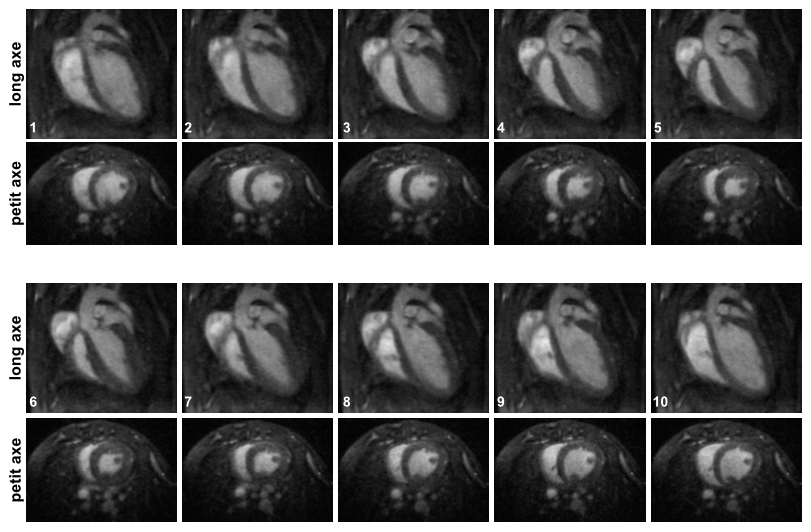
\includegraphics[scale=0.5]{./figure/chap6/Fig8.png}
\caption[Mesure linéarité du flux]{\label{fig:FluxFantLinear} Mesure des vitesses sur un fantôme de flux effectuée avec une séquence FLASH et UTE en fonction de la vitesse du flux imposé dans le tube (0.497, 0.400, 0.306, 0.197, 0.095 m/s) avec une concentration en $\text{MnCl}_2$ de 2 mM et une valeur de VENC de 1.0 m/s.}
\line(1,0){400} \\ 
\end{figure}


\section{Résultats préliminaires \textit{in-vivo}}

L'imagerie des souris a été effectuée à 7 Tesla avec une antenne surfacique à 4 éléments et les paramètres suivants :
TR/TE = 3.5/0.45 ms, type d'excitation radiofréquence/durée/angle d'excitation = bp32/0,05 ms/15$\degres$, champ de vue = 20 x 20 x 20, matrice = 128 x 128 x 128, nombre de volume ciné = 10, nombre de projection  = 18140, bande passante de réception = 100 kHz, VENC = 1.2 m/s, temps d'acquisition total $\approx$ 45 minutes.

Les souris sont anesthésiées avec 1$\%$ d'isoflurane dans l'air. Le signal ECG est récupéré grâce à des électrodes positionnées la patte supérieure droite et la patte inférieure gauche. Le signal est utilisé pour synchroniser l'acquisition aux battements de coeur grâce à un système de visualisation et de synchronisation spécifique (SA Instruments, Inc., NY). L'ECG est visualisé sur l'interface et le rythme cardiaque est stabilisé entre 400 et 415 battements par minute en modifiant le pourcentage d'isoflurane inhalé. 100 $\mu L$ de Sinerem sont injecté par la veine caudale de la souris à une concentration de 200 $\mu mol$ Fe/kg.

\subsection{Validation de la séquence}

La séquence a été appliquée sur plusieurs souris C57/Black 6 (27-32g). Des images coronales représentatives sont montrées sur la figure \ref{fig:CarteVitesse} qui sont reconstruites à partir d'une même expérience. Les images en magnitudes sont reconstruites à partir des données d'une seule direction d'encodage de vitesse.  On observe que la combinaison entre l'injection de l'agent de contraste à base de nanoparticule de fer et l'utilisation d'une séquence à temps d'écho court permet d'obtenir un bon signal-sur-bruit du sang de 35.5 $\pm$ 2.3 ce qui est particulièrement important en imagerie de phase car le bruit sur les cartes de vitesse est inversement proportionnel au signal-sur-bruit des tissus. 

De plus, l'agent de contraste étant restreint au système vasculaire, le contraste entre le myocarde et le sang est important. Cela permet donc à partir d'utiliser l'acquisition de mesure de flux pour obtenir des informations anatomique et fonctionnelles (fraction d'éjection, volume d'éjection etc) mais aussi de pouvoir segmenter les cartes de vitesse à partir de l'image en magnitude. C'est un atout important de cette méthode puisque les erreurs provoquées par exemple par des arythmies ou des mouvements impactent aussi les images anatomiques.

Un autre point intéressant est la très bonne homogénéité du signal sanguin que ce soit dans les cavités cardiaques ou bien dans la crosse aortique et cela tout au long du cycle cardiaque et surtout malgré la présence des gradients d'encodage de vitesse. Cela permet d'obtenir des informations de vitesse dans tout le système cardiovasculaire en particulier dans les régions comme la crosse aortique avec des flux rapides (voir carte de vitesse).

La résolution temporelle de 14 ms, correspondant aux 4 signaux IRM avec un encodage de vitesse différent, permet d'obtenir une visualisation suffisante des modifications de vitesse au cours du cycle cardiaque et la résolution spatiale des images (< 200 $\mu m$) permet d'obtenir des informations de vitesse dans la plupart des vaisseaux et en particulier dans les artères pulmonaires qui est une information importante dans le cas de plusieurs pathologie et en particulier pour l'hypertension pulmonaire.

\begin{figure}[H]
\centering
\line(1,0){400} \\
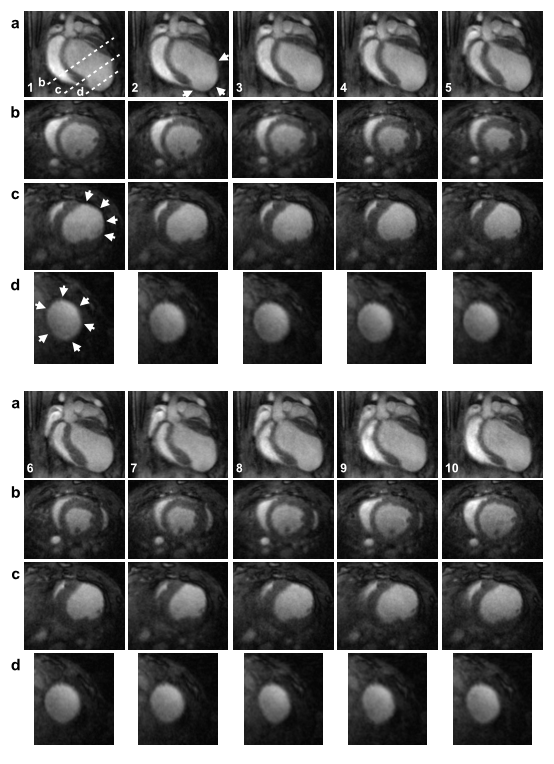
\includegraphics[scale=0.7]{./figure/chap6/Fig9.png}
\caption[Carte de vitesse]{\label{fig:CarteVitesse} Images coronales en magnitude, carte de vitesse selon la direction X, Y et Z et carte de vitesse absolue d'une acquisition représentative reconstruites à partir du même jeu de donnée.}
\line(1,0){400} \\ 
\end{figure}

\subsection{Quantification préliminaire des vitesses sur un modèle d'hypertension artérielle pulmonaire}

5 souris mâle OB1 ont été imagées OB1 (35-40g) durant cette étude, dont 3 d'entre elles ont développées une hypertension artérielle pulmonaire (HTAP) après avoir passé 21 jours dans un caisson hypobare à une pression de 50 kPa.
Les vitesses ont été mesurées dans la crosse aortique et une des artères pulmonaires, les résultats sont présentées dans la figure \ref{fig:CarteVitesse}. On observe que les vitesses maximums mesurées au cours du cycle cardiaque chez les souris HTAP ($v = 30,3 \pm 5,7$) sont plus faibles que chez les souris contrôles ($v = 54,0 \pm 2,8$) en particulier au niveau de l'artère pulmonaire.

La diminution de vitesse des flux dans sur les modèles HTAP a déjà été observée dans une précédente étude réalisée sur le rat \cite{Dumas2011effect} avec la stratégie d'angiographie par résonance magnétique dynamique cartésienne présentée dans le chapitre \ref{Chap3}. De plus, ils ont montré la consistance de leurs données avec d'autres travaux qui ont étudiés la pression sanguine et le débit cardiaque \cite{pozeg2003vivo,hessel2006characterization}.

\begin{figure}[H]
\centering
\line(1,0){400} \\
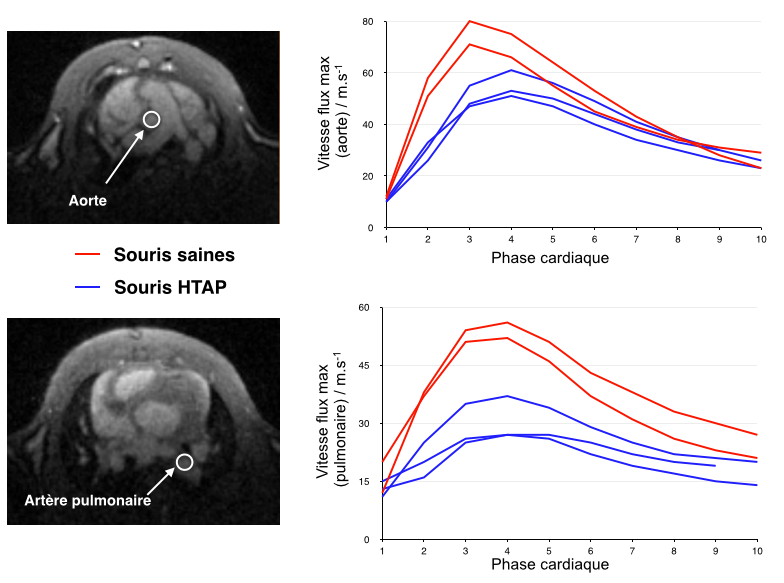
\includegraphics[scale=0.7]{./figure/chap6/Fig10.png}
\caption[Vitesse HTAP]{\label{fig:CarteVitesse} Schéma présentant les mesures des vitesses maximum effectuées chez 3 souris ayant développées un syndrôme HTAP et 2 souris saines. Les mesures ont été effectuées au niveau de l'aorte pour le schéma du haut et sur une artère pulmonaire sur le schéma du bas dont les positions sont illustrées sur les images à gauche.}
\line(1,0){400} \\ 
\end{figure}

\section{Discussion}

L'imagerie 4D de flux basée sur le principe du contraste de phase est une stratégie en pleine explosion \cite{Stankovic:2014aa,Garcia:2014aa,Petersson:2015aa} pour des applications cardiovasculaires grâce aux différentes méthodes qui ont été développées que ce soit pour réduire le temps d'acquisition des séquences \cite{Liu:2014aa} ou en terme d'analyse des données \cite{Eriksson:2010aa}. Cependant cet intérêt est pour le moment restreint à l'imagerie clinique, la plupart des travaux publiés sur le petit animal utilisent encore des acquisition 2D \cite{Zhao:2009ng}. 
L'objectif dans cette partie a été le développement d'une méthode robuste 4D permettant d'obtenir des mesures précises pour l'imagerie en 3D des flux du système cardiovasculaire chez le petit animal.

Le rehaussement par injection d'un agent de contraste intravasculaire a deux avantages. Le premier est qu'il permet d'améliorer le rapport signal-sur-bruit des images en magnitude et de réduire le bruit sur les cartes de vitesse car celui-ci est inversement proportionnel au signal-sur-bruit. Bock et al \cite{Bock:2010aa} ont montré que l'amélioration du signal a permi chez l'humain d'améliorer la visualisation des flux sanguin grâce aux trajectoires des particules. 
Le deuxième avantage est qu'il permet d'obtenir un très bon contraste-sur-bruit entre le sang les tissus environnants (myocarde, poumon, muscle etc) et permet donc de segmenter les données de phase à partir des données en magnitude.  En effet, sans injection le signal du sang est faible à cause de l'absence d'effet temps-de-vol en imagerie 3D cardiaque. L'alternative généralement utilisé est l'utilisation des images de contraste de phase mais celles-ci ne permettent pas de visualiser précisément l'interface sang/tissus à cause de la réduction de la vitesse et donc du contraste au bord des vaisseaux. La précision dans le cas de mesure de débit ou de vitesse moyenne a donc de grande chance d'être améliorée avec l'injection d'agents de contraste intravasculaire.

L'utilisation d'une séquence avec une trajectoire UTE et de gradients bipolaires intenses permet d'atteindre des temps d'écho inférieur à 0,6 ms. Cela permet d'une part d'obtenir un signal positif avec les agents de contraste à base de nanoparticules de fer mais aussi permet de réduire la sensibilité de la séquence aux artéfacts de flux. Cela est confirmé par l'étude \textit{in-vitro} réalisée sur un fantôme de flux dont les mesures de vitesses obtenues avec la séquence UTE montrent une très faible dispersion et sont cohérents avec les vitesses de flux imposées.
%Les mesures de flux effectuées sur fantôme montrent que la séquence UTE développée permet d'obtenir des résultats en accord avec les vitesses imposées à l'intérieur du tube et que ces mesures sont robustes à l'augmentation de la concentration en $\text{MnCl}_2$. Alors que l'on observe que les mesures avec la séquence cartésienne montre une bien plus grande variabilité qui peut s'expliquer par l'augmentation de l'effet $T_2*$ avec la concentration. Cependant même lorsque la concentration en $\text{MnCl}_2$ est nulle, la variabilité est plus importante, cela peut être dû à l'aspect pulsatile du flux  provoqué par la pompe à laquelle la séquence cartésienne est plus sensible.

Dans la littérature, seuls deux études font état de l'utilisation d'une méthode 4D de mesure de flux par contraste de phase chez la souris. Janiczek et al \cite{Janiczek:2011qm} utilisent une trajectoire de 3D type Stack-Of-Star spiral qui dispose aussi de propriété de robustesse vis-à-vis des artefacts de flux dans les zones tortueuses comparée à une séquence cartésienne 2D. Cependant ceux-ci n'utilisent que très peu la possibilité d'accélération de la séquence spiral car le temps d'acquisition pour leurs expériences (42 à 53 minutes en fonction du rythme cardiaque de leurs animaux) est de l'ordre de celle de nos expériences pour une résolution spatiale isotropique approximativement égale mais un champs-de-vue dans la dernière dimension 4 fois plus faible (< à 5,5 mm). Le champ-de-vue est centré sur la crosse aortique pour obtenir un effet temps-de-vol dans le sang et donc des mesures précises du sang.

A notre connaissance Bovenkamp et al \cite{bovenkamp2014velocity} sont les seuls à avoir appliquée une méthode de mesure de flux 4D sur le coeur entier chez la souris. Leur étude est basée sur l'utilisation d'une séquence cartésienne sans injection d'agent de contraste. Le faible signal sanguin dû à l'absence d'effet temps-de-vol en imagerie 3D ainsi que la diminution du signal supplémentaire provoquée par des temps d'écho important de 2,2 ms explique le choix d'utiliser une faible résolution spatiale pour leurs images ($140 \times 200 \times 500 \mu$) ainsi d'un nombre d'accumulation de 3 pour obtenir un signal-sur-bruit suffisant. Cela augmente considérablement le temps d'acquisition de leurs expériences à des valeurs d'environ une heure.

Il est a noté que les deux méthodes décrites dans la littérature permettent d'atteindre des résolutions temporelles inférieur d'un facteur deux à notre stratégie. Cependant notre méthode d'encodage rend la reconstruction très flexible puisqu'il est possible d'atteindre des résolutions temporelles de 7 ms ou bien de 3,5 ms à partir du même jeu de donnée en utilisant la même stratégie décrite dans le chapitre \ref{Chap4} permettant d'obtenir les images avec une forte résolution temporelle à partir de jeu de donnée avec une forte résolution spatiale. Cela aura bien entendu des conséquences sur la résolution effective de l'image mais  la trajectoire radiale peut supporter de fort facteur de sous-échantillonnage comme expliquée dans le chapitre \ref{Chap2}. Cette stratégie peut donc être envisagée pour la quantification de vitesse dans les vaisseaux de tailles importantes en complément de la quantification avec une résolution temporelle plus faible dans les vaisseaux de faibles diamètres.

La stratégie développée dans ce chapitre semble donc particulièrement intéressante pour sa faible sensibilité aux déphasages provoquées par les flux turbulents, sa capacité à visualiser les flux dans tout le système cardiovasculaire y compris les cavités cardiaques ainsi que la possibilité d'obtenir en une acquisition des informations anatomiques et fonctionnelles. La résolution spatiale et le signal-sur-bruit des images est supérieures aux autres méthodes décrites dans la littérature pour des champs-de-vue plus important et des temps d'acquisitions plus court. L'utilisation de cette méthode semble donc très prometteuse en particulier dans le cadre du phénotypage ou d'études de pathologie chez le petit animal dans lesquelles les modifications de vitesses sont diffuses comme des modèles d'artérioscléroses ou d'hypertension et qui requiert l'imagerie et des mesures de vitesse dans des champ-de-vue important


\section{Perspectives}

Un certain nombre de développement sont à effectuer sur le traitement des données dans le cadre de la publication ce travail. En effet, il est nécessaire de mettre en place un protocole d'analyse des données de flux permettant l'extraction des vitesse moyennes ou maximum dans les vaisseaux ou bien pour la visualisation et la quantification des trajectoires des flux.

Ces développements permettront une analyse plus précise de l'effet du sous-échantillonnage des données sur la mesure des vitesses car celui-ci a un effet sur la résolution spatiale effective des images qui modifiera certainement la vitesse dans les vaisseaux. Mais, dans le cas de la mesure des flux maximum dans la crosse aortique ou l'artère pulmonaire, il est possible que ce paramètre quantitaif soit faiblement sensible à la baisse de résolution spatiale et qu'il puisse être exploité avec des acquisitions sous-échantillonnées et donc des temps d'acquisitions plus réduit.

De même, une partie du travail restant est de quantifier l'effet de l'augmentation de la résolution temporelle des données. Par exemple en comparant les trajectoires des flux avec un même jeu de donnée reconstruit avec une résolution temporelle de 14 ms et une résolution temporelle de 10,5/7/3,5 ms ainsi que les vitesses moyennes et maximum  mesurées tout d'abord \textit{in-vitro} sur des fantômes de flux incurvé puis potentiellement \textit{in vivo}.

Toutes ces perspectives sont en cours d'évaluation et les résultats seront amenée à être soumis prochainement.